\chapter{Previous work}

\section{The reconstruction of the Assembly history of the Milky Way}
Inferring the assembly history of the Milky Way is a challenging task, even in the era of the astrometric Gaia mission and its 6 dimensional 
phase space data, and the complementary chemical information obtained from the wide-field spectroscopic programs such as the GALAH survey
\cite{desilvaGALAHSurveyScientific2015}, the H3 survey \cite{conroyMappingStellarHalo2019}, APOGEE \cite{majewskiApachePointObservatory2017}, RAVE \cite{steinmetzRadialVelocityExperiment2006},  SEGUE \cite{yannySEGUESPECTROSCOPICSURVEY2009}, and 
LAMOST \cite{cuiLargeSkyArea2012}. The dynamical times of the accreted objects are far longer than the age of the host galaxy, allowing the 
phase space to retain part of the information on the original orbit parameters. On the other hand, the chemical space is dependent on the star formation history, in particular type II SNe produce $\alpha$-elements and iron with a almost constant ratio, while type Ia SNe produce more efficiently iron. Another factor that governs the chemical space is the total mass of the galaxy, since the more massive galaxies are more capable to resist the expulsion of metals due to feedback mechanism. The crossmatch between Gaia and spectroscopic data allowed for the discovery of the "Gaia-Sausage-Enceladus" (GSE) (\cite{belokurovCoformationDiscStellar2018}, \cite{helmiMergerThatLed2018}), a massive accretion event whose remnant now dominates the observation of the inner stellar halo of our Galaxy. 
\begin{figure}[ht]
    \centering
    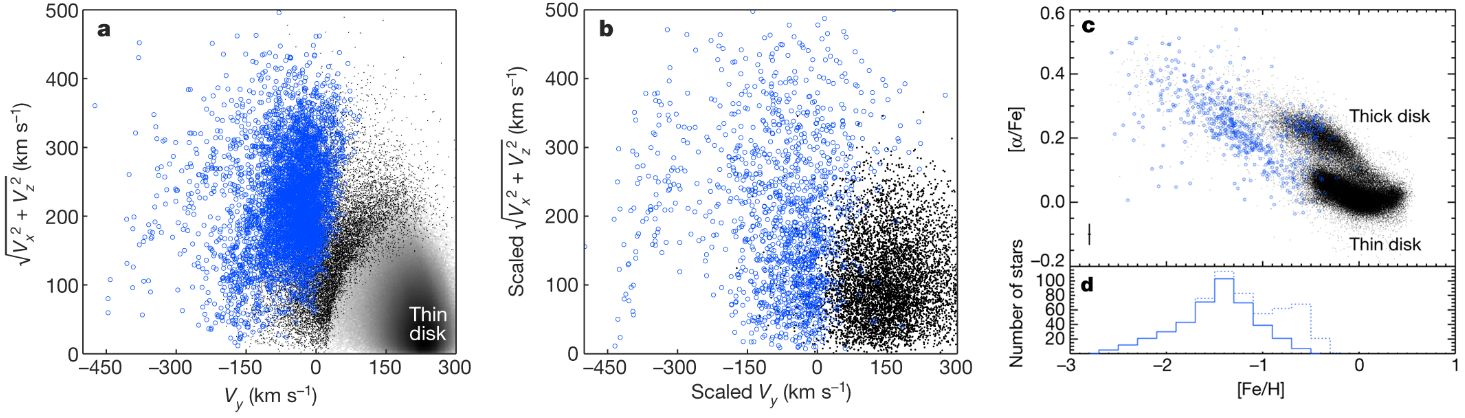
\includegraphics[width=1\textwidth]{./figure/Gaia_Helmi18.png}
    \caption{Gaia DR2 data with APOGEE abundance measurement. In blue are reported the eccentric stars that were selected and crossmatch in \cite{helmiMergerThatLed2018}.}
    \label{fig:sbi_approaches}
\end{figure}



Robustly identify distinct structure is challenging, and disentangle the components in fully phase mix situations is nearly impossible. In order to characterize the assembly history \cite{cunninghamReadingCARDsImprint2022}
propose to use the "CARDs", the chemical abundance ratio distributions of the stars, obtained from the FIRE-2 zoom-in cosmological simulations of MW-mass galaxies \cite{wetzelRECONCILINGDWARFGALAXIES2016}.
Although similar to CASBI in how to leverage N-body simulations, this method do not recovers posteriors for the parameters of the accreted objects, but rather considers the host halo as a linear combinations of templates CARDs, treating each coefficient as the fraction of mass contribution from the accretion event, and tries to recover those coefficients by maximize a loss that compares the observed CARDs with the combination of the templates. This method and CASBI share two more similarities: 1. Both of these methods are meant to be used on simulations, and the integrations of observational data is not yet implemented, even though theoretically possible. 2. Both rely on the assumption that the chemical space of accreted and isolated dwarf galaxies is very similar, due to ram pressure quenching the star formation history of the accreted object and hence 'freezing' these abundance ratios at the infall time. This assumption is investigated further in section 6 of \cite{cunninghamReadingCARDsImprint2022}. 
Another approach is presented in \cite{deasonUnravellingMassSpectrum2023}, which takes advantage of the mass-metallicity relation to decompose the metallicity distribution functions (MDF) of the host galaxy as a mixture of accreted halo's MDF, assumed gaussian for each of these building blocks. The objective of this work is to obtain a posterior distribution for the number of galaxies in each luminosity bin, which can be considered a proxy for the star mass. In CASBI we adopt the same superimposition philosophy of the components contribution, but we do not assume neither a prefix or an analytical form for the joint distribution of the chemical abundance, relaxing these assumption and relying only on the available samples from the N-body simulations.  